\documentclass[9pt,a4paper,twocolumn,twoside]{tau-class/tau}
\usepackage[utf8]{inputenc}
\usepackage[slovene]{babel}
\usepackage{amsmath}
\usepackage{graphicx}
\usepackage{booktabs}
\usepackage{listings}

% Komanda za vrednost z aboslutno napako
\newcommand{\abserr}[5]{
    \ensuremath{#1_{#2} = (#3 \ \pm \ #4) \ #5}
}

\newcommand{\relerr}[5]{
    \ensuremath{#1_{#2} = #3 \ (1 \pm \ #4) \ #5}
}

\newcommand{\relativna}[3]{
    \ensuremath{#1 \ (1 \pm #2) \ #3}
}

\newcommand{\absolutna}[3]{
    \ensuremath{(#1 \ \pm \ #2) \ #3}
}


%----------------------------------------------------------
% TITLE
%----------------------------------------------------------

\journalname{Fizikalni eksperimetni III}
\title{Optična rotacija raztopine saharoze}

%----------------------------------------------------------
% AUTHORS, AFFILIATIONS AND PROFESSOR
%----------------------------------------------------------

\author[a]{Matija Zanjkovič}
\affil[a]{Univerza v Mariboru, Fakulteta za naravoslovje in matematiko}


%----------------------------------------------------------
% FOOTER INFORMATION
%----------------------------------------------------------

\institution{Univerza v Mariboru, Fakulteta za naravoslovje in matematiko}
\footinfo{Projektna naloga}
\theday{Julij 2025}
\leadauthor{Zanjkovič Matija}
\author[a]{Mesarec Tilen}
\author[a]{Petauer Maja}
\course{Fizikalni eksperimenti III}

%----------------------------------------------------------
% ABSTRACT AND KEYWORDS
%----------------------------------------------------------

\begin{abstract}
V tej nalogi smo merili optično rotacijo polarizirane svetlobe v raztopinah saharoze različnih koncentracij pri dveh valovnih dolžinah (rdeča in zelena). Iz podatkov smo izračunali specifično rotacijo, ocenili napake in analizirali odvisnost od valovne dolžine z Drudejevo enačbo.
\end{abstract}

\keywords{specifična rotacija, saharoza, Drudejeva enačba, med}

%----------------------------------------------------------

\begin{document}
\setlength{\parindent}{0pt}
        
    \maketitle 
    \thispagestyle{firststyle} 
    \tauabstract 

%----------------------------------------------------------
\section{Uvod}

\taustart{O}ptična rotacija je pojav, kjer kiralne molekule, kot je saharoza, zavrtijo ravnino polarizirane svetlobe. Ta pojav je odvisen od koncentracije snovi $c$, dolžine poti svetlobe $l$ in valovne dolžine $\lambda$. Namen vaje je določiti specifično rotacijo pri različnih koncentracijah in valovnih dolžinah ter preveriti Drudejev model disperzije.

%----------------------------------------------------------
\section{Teorija}

Kot rotacije $\alpha$ je povezan s specifično rotacijo $[\alpha]_\lambda$ preko:
\[
\alpha(\lambda) = [\alpha]_\lambda \cdot c \cdot l
\]
Specifična rotacija je funkcija valovne dolžine in jo lahko približamo z Drudejevim modelom:
\[
[\alpha](\lambda) = \frac{k \lambda^2}{\lambda^2 - A^2}
\]
kjer sta $k$ in $A$ parametra, ki ju določimo iz eksperimentalnih podatkov.

%----------------------------------------------------------
\section{Merjene količine}

\begin{itemize}
    \item \textbf{Koncentracija saharoze} $c$ (g/mL)
    \item \textbf{Valovna dolžina} $\lambda$ (nm),
    \item \textbf{Kot rotacije} $\alpha$ (°), 
    \item \textbf{Dolžina cevi} $l$ (dm)
\end{itemize}


%----------------------------------------------------------
\section{Meritve}

% Dolžina cevi
Dolžina cevi:
\[
\abserr{L}{}{11.5}{0.5}{\text{dm}}
\]
\[
\relerr{L}{}{11.5}{0.043}{\text{dm}}
\]

% Volumen raztopine
Volumen raztopine je bil:
\[
\abserr{V}{}{3000}{60}{\text{mL}}
\]
\[
\relerr{V}{}{3000}{0.02}{\text{mL}}
\]

To smo počeli pri konstantni temperaturi $T = 22 \pm 1 \, \text{°C}$, saj 
na specifično rotacijo vpliva tudi temperatura.\\\\

% Masa saharoze
Masa saharoze je bila izmerjena z napako $3\,\text{g}$. Relativna napaka koncentracije:

\begin{table}[H]
\centering
\begin{tabular}{ccc}
\toprule
$c$ [g/mL] & $\sigma c$ \\
\midrule
0.030 & 0.033 \\
0.050 & 0.020 \\
0.070 & 0.014 \\
0.090 & 0.011 \\
0.100 & 0.010 \\
\bottomrule
\end{tabular}
\caption{Relativna napaka koncentracije raztopine saharoze.}
\end{table}


\begin{table}[H]
\centering
\begin{tabular}{cccccc}
\toprule
$c$ [g/mL] & $\alpha_r$ [°] & $\alpha_z$ [°]  & $\Delta \alpha$ [°] & $\sigma \alpha_r$ & $\sigma \alpha_z$ \\
\midrule
0.030 & 22 & 23 & 2 & 0,09 & 0,09 \\
0.050 & 34 & 37 & 2 & 0,06 & 0,05 \\
0.070 & 47 & 53 & 2 & 0,04 & 0,04 \\
0.090 & 63 & 63 & 2 & 0,03 & 0,03 \\
0.100 & 69 & 70 & 2 & 0,03 & 0,03 \\
\bottomrule
\end{tabular}
\caption{Koti rotacije za rdečo ($\alpha_r$) in zeleno ($\alpha_z$) svetlobo.}
\end{table}


%----------------------------------------------------------
\section{Izračun specifične rotacije}

Specifična rotacija $[\alpha]$ za vsako meritev:
\[
[\alpha] = \frac{\alpha}{c \cdot L}
\]

\begin{minipage}{0.24\textwidth}
\textbf{Rdeča:}
\begin{align*}
[\alpha]_{c=0.030} &= 64 \ (1 \pm 0{,}19) \ \frac{^\circ \cdot \mathrm{mL}}{\mathrm{g} \cdot \mathrm{dm}}\\
[\alpha]_{c=0.050} &= 59 \ (1 \pm 0{,}14) \ \frac{^\circ \cdot \mathrm{mL}}{\mathrm{g} \cdot \mathrm{dm}}\\
[\alpha]_{c=0.070} &= 58 \ (1 \pm 0{,}12) \ \frac{^\circ \cdot \mathrm{mL}}{\mathrm{g} \cdot \mathrm{dm}}\\
[\alpha]_{c=0.090} &= 61 \ (1 \pm 0{,}11) \ \frac{^\circ \cdot \mathrm{mL}}{\mathrm{g} \cdot \mathrm{dm}}\\
[\alpha]_{c=0.100} &= 60 \ (1 \pm 0{,}10) \ \frac{^\circ \cdot \mathrm{mL}}{\mathrm{g} \cdot \mathrm{dm}}\\
\end{align*}
\end{minipage}
\hfill
\begin{minipage}{0.24\textwidth}

\begin{align*}
[\alpha]_{c=0.030} &= (64 \pm 12) \ \frac{^\circ \cdot \mathrm{mL}}{\mathrm{g} \cdot \mathrm{dm}}\\
[\alpha]_{c=0.050} &= (59 \pm 8) \ \frac{^\circ \cdot \mathrm{mL}}{\mathrm{g} \cdot \mathrm{dm}}\\
[\alpha]_{c=0.070} &= (58 \pm 7) \ \frac{^\circ \cdot \mathrm{mL}}{\mathrm{g} \cdot \mathrm{dm}}\\
[\alpha]_{c=0.090} &= (61 \pm 7) \ \frac{^\circ \cdot \mathrm{mL}}{\mathrm{g} \cdot \mathrm{dm}}\\
[\alpha]_{c=0.100} &= (60 \pm 6) \ \frac{^\circ \cdot \mathrm{mL}}{\mathrm{g} \cdot \mathrm{dm}}\\
\end{align*}
\end{minipage}

\[
\overline{[\alpha]_{r}}  = (60 \ \pm \ 9)  \frac{^\circ \cdot \mathrm{mL}}{\mathrm{g} \cdot \mathrm{dm}}
\]
\[
\overline{[\alpha]_{r}} = 60 \ (1 \pm 0{,}15) \ \frac{^\circ \cdot \mathrm{mL}}{\mathrm{g} \cdot \mathrm{dm}}
\]

\vspace{1em}

\begin{minipage}{0.24\textwidth}
\textbf{Zelena:}
\begin{align*}
[\alpha]_{c=0.030} &= (67 \pm 12) \ \frac{^\circ \cdot \mathrm{mL}}{\mathrm{g} \cdot \mathrm{dm}}\\
[\alpha]_{c=0.050} &= (64 \pm 9) \ \frac{^\circ \cdot \mathrm{mL}}{\mathrm{g} \cdot \mathrm{dm}}\\
[\alpha]_{c=0.070} &= (66 \pm 8) \ \frac{^\circ \cdot \mathrm{mL}}{\mathrm{g} \cdot \mathrm{dm}}\\
[\alpha]_{c=0.090} &= (61 \pm 7) \ \frac{^\circ \cdot \mathrm{mL}}{\mathrm{g} \cdot \mathrm{dm}}\\
[\alpha]_{c=0.100} &= (61 \pm 6) \ \frac{^\circ \cdot \mathrm{mL}}{\mathrm{g} \cdot \mathrm{dm}}\\
\end{align*}
\end{minipage}
\hfill
\begin{minipage}{0.24\textwidth}
\begin{align*}
[\alpha]_{c=0.030} &= 67 \ (1 \pm 0{,}18) \ \frac{^\circ \cdot \mathrm{mL}}{\mathrm{g} \cdot \mathrm{dm}}\\
[\alpha]_{c=0.050} &= 64 \ (1 \pm 0{,}14) \ \frac{^\circ \cdot \mathrm{mL}}{\mathrm{g} \cdot \mathrm{dm}}\\
[\alpha]_{c=0.070} &= 66 \ (1 \pm 0{,}12) \ \frac{^\circ \cdot \mathrm{mL}}{\mathrm{g} \cdot \mathrm{dm}}\\
[\alpha]_{c=0.090} &= 61 \ (1 \pm 0{,}11) \ \frac{^\circ \cdot \mathrm{mL}}{\mathrm{g} \cdot \mathrm{dm}}\\
[\alpha]_{c=0.100} &= 61 \ (1 \pm 0{,}10) \ \frac{^\circ \cdot \mathrm{mL}}{\mathrm{g} \cdot \mathrm{dm}}\\
\end{align*}
\end{minipage}

\[
\overline{[\alpha]_{z}} = (64 \ \pm \ 10) \frac{^\circ \cdot \mathrm{mL}}{\mathrm{g} \cdot \mathrm{dm}}
\]
\[
\overline{[\alpha]_{z}} = 64 \ (1 \pm 0{,}16) \ \frac{^\circ \cdot \mathrm{mL}}{\mathrm{g} \cdot \mathrm{dm}}
\]
%----------------------------------------------------------
\pagebreak

\section{Analiza: Drudejev model}

Ker smo specifično rotacijo $[\alpha](\lambda)$ merili pri dveh različnih valovnih dolžinah, smo podatkom prilegli Drudejevo enačbo, ki opisuje odvisnost specifične rotacije od valovne dolžine $\lambda$:
\[
[\alpha](\lambda) = \frac{k \lambda^2}{\lambda^2 - A^2}
\]

Parametra $k$ in $A$ smo določili numerično.


Rezultati prileganja:
\begin{align*}
\abserr{k}{}{53,88}{2,82}{} \\
\relerr{k}{}{55,88}{0,05}{} \\\\
\noindent \abserr{A}{}{209,00}{35}{} \\
\relerr{A}{}{209,00}{0,17}{}
\end{align*}

\begin{figure}[H]
    \centering
    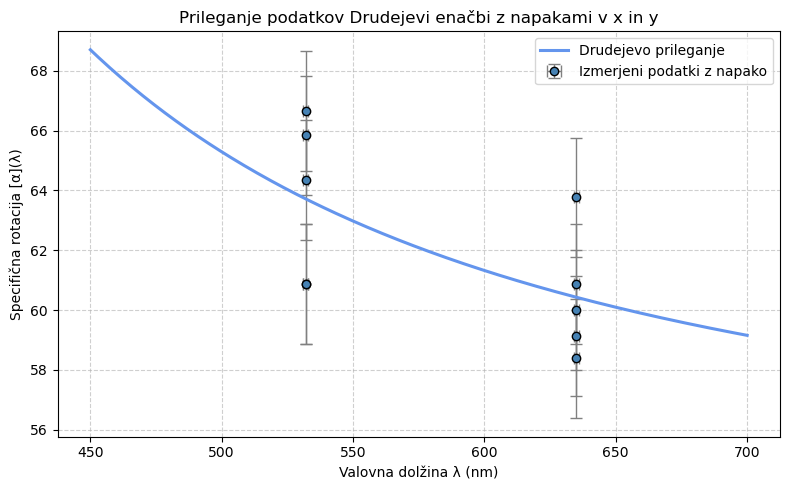
\includegraphics[width=0.9\linewidth]{output.png}
    \caption{Prileganje Drudejeve enačbe eksperimentalnim podatkom specifične rotacije.}
    \label{fig:specrot}
\end{figure}

\subsection{Napake in rezultati}

% Rdeči laser (635 nm)
\textbf{Rdeči laser (635 nm):}
\begin{align*}
\abserr{[\alpha]}{635\,\text{nm}}{60}{10}{} \frac{^\circ \cdot \mathrm{mL}}{\mathrm{g} \cdot \mathrm{dm}}\\
\relerr{[\alpha]}{635\,\text{nm}}{60}{0,17}{} \frac{^\circ \cdot \mathrm{mL}}{\mathrm{g} \cdot \mathrm{dm}}\\
\end{align*}

% Zeleni laser (532 nm)
\textbf{Zeleni laser (532 nm):}
\begin{align*}
\abserr{[\alpha]}{532\,\text{nm}}{64}{10}{} \frac{^\circ \cdot \mathrm{mL}}{\mathrm{g} \cdot \mathrm{dm}}\\
\relerr{[\alpha]}{532\,\text{nm}}{64}{0,16}{} \frac{^\circ \cdot \mathrm{mL}}{\mathrm{g} \cdot \mathrm{dm}}\\
\end{align*}

% Modri laser (450 nm)
\textbf{Modri laser (450 nm):}
\begin{align*}
\abserr{[\alpha]}{450\,\text{nm}}{69}{10}{} \frac{^\circ \cdot \mathrm{mL}}{\mathrm{g} \cdot \mathrm{dm}}\\
\relerr{[\alpha]}{450\,\text{nm}}{62}{0,14}{} \frac{^\circ \cdot \mathrm{mL}}{\mathrm{g} \cdot \mathrm{dm}}
\end{align*}



\section*{Med}

S pomočjo znanja o specifični rotaciji glukoze in fruktoze smo se odločili, da bomo primerjali dva meda in poskušali ugotoviti, ali sta naravna ali z dodatki.

Naravni med je sestavljen predvsem iz glukoze in fruktoze in sicer v razmerju $36:41$. Specifične rotacije glukoze in fruktoze pri $T = 20 \,^\circ$C in $\lambda = \ 589 $ nm sta:

\begin{align*}
[\alpha]_{glukoza} &= 53 \ \frac{^\circ \cdot \mathrm{mL}}{\mathrm{g} \cdot \mathrm{dm}} \\
[\alpha]_{fruktoza} &= -92 \ \frac{^\circ \cdot \mathrm{mL}}{\mathrm{g} \cdot \mathrm{dm}} \\
\end{align*}

Kar pomeni, da je specifična rotacija medu:
\[
[\alpha]_{med_1} = \frac{36 \cdot [\alpha]_{glukoza} + 41 \cdot [\alpha]_{fruktoza}}{36 + 41} = -24 \ \frac{^\circ \cdot \mathrm{mL}}{\mathrm{g} \cdot \mathrm{dm}}
\]

Glede na raziskavo pa naj bi bila specifična rotacija sintetičnega medu bila zaradi dodanih sladkorjev s pozitivno kiralnostjo v rangu: $7 - 89 \ \frac{^\circ \cdot \mathrm{mL}}{\mathrm{g} \cdot \mathrm{dm}}$ \href{https://doi.org/10.3390/molecules27248916}{[1]}

Merili smo dva cvetlična meda, en je bil domač, drugi pa kupljen.

\[
    [\alpha]_{med_1} = \frac{\alpha}{c \cdot L} = \frac{-4}{0.010 \cdot 11.5} = -35 \ \frac{^\circ \cdot \mathrm{mL}}{\mathrm{g} \cdot \mathrm{dm}}
\]
\[
    \sigma [\alpha]_{med_1} = 0,2 + 0,5 + 0,04 = 0,74
\]

\begin{center}
\fbox{
    \begin{minipage}{0.4\textwidth}
        Rezultat za specifično rotacijo medu:
        \[
            \abserr{[\alpha]}{med_1}{-35}{26}{\frac{^\circ \cdot \mathrm{mL}}{\mathrm{g} \cdot \mathrm{dm}}}
        \]
        \[
            \relerr{[\alpha]}{med_1}{-35}{0,74}{\frac{^\circ \cdot \mathrm{mL}}{\mathrm{g} \cdot \mathrm{dm}}}
        \]
    \end{minipage}
}
\end{center}

Vidimo, da je specifična rotacija medu precej nižja od pričakovane vrednosti za naravni med, ampak je tudi napaka ogromna. Vendar je naš med bil cvetlični med,
ki ima glede na raziskavo specifično rotacijo manjšo kot ostali medi. 


Pri drugem medu (iz trgovine) pa smo dobili rezultat:

\[
    [\alpha]_{med_2} = \frac{\alpha}{c \cdot L} = \frac{3}{0.005 \cdot 11.5} = 52 \ \frac{^\circ \cdot \mathrm{mL}}{\mathrm{g} \cdot \mathrm{dm}}
\]
\[
    \sigma [\alpha]_{med_2} = 0,2 + 0,5 + 0,04 = 0,74
\]

\begin{center}
\fbox{
    \begin{minipage}{0.4\textwidth}
        Rezultat za specifično rotacijo drugega medu:
        \[
            \abserr{[\alpha]}{med_2}{52}{38}{\frac{^\circ \cdot \mathrm{mL}}{\mathrm{g} \cdot \mathrm{dm}}}
        \]
        \[
            \relerr{[\alpha]}{med_2}{52}{0,74}{\frac{^\circ \cdot \mathrm{mL}}{\mathrm{g} \cdot \mathrm{dm}}}
        \]
    \end{minipage}
}
\end{center}

%----------------------------------------------------------
\section{Zaključek}

Eksperiment je pokazal, da se optična rotacija saharoze v vodi spreminja z različnimi koncentracijami in valovnimi dolžinami. 
Izračunana specifična rotacija potrjuje teorijo o optični aktivnosti, ki smo jo nato opisali z Drudejevim modelom.
Primerjali smo tudi dva različna meda v grobem je med z negativno specifično rotacijo naraven, med s pozitivno pa z dodatki.

%----------------------------------------------------------
 \begin{thebibliography}{9}

    \bibitem{gerginova2022optical}
    D. Gerginova, V. Kurteva, S. Simova,
    \textit{Optical Rotation—A Reliable Parameter for Authentication of Honey?},
    Molecules, 27(24), 8916, 2022.

    \bibitem{advanced_organic_chemistry}
    Advanced Organic Chemistry Part A: Structure and Mechanisms Part B: Reactions and Synthesis, Chemistry International, vol. 24, no. 5, pp. 28-29, Sep. 2002, doi: 10.1515/ci.2002.24.5.28b.

    \bibitem{lei2018optimized}
    Y. Lei, H. Jia, X. Xu, and S. Jiang,
    "An Optimized Drude's Equation For Polarization Measurement in the Visible Region and Concentrations Estimation,"
    \textit{IEEE Photonics Journal}, vol. 10, no. 1, pp. 1-9, Feb. 2018, Art no. 6100209,
    doi: 10.1109/JPHOT.2017.2787576.

\end{thebibliography}

\end{document}